\section*{Tag 19 — Datamatrix komplett von Hand}

Diese Lösung ist als \emph{Quervergleich} angelegt: an jeder Stelle
darfst du einsteigen, ohne den Anschluss zu verlieren. Die
Checkpoints~A--G für „MUT" und A'--G' für „GESCHAFFT" sind nummeriert,
sodass du sagen kannst: „Bis B passt alles, ab C habe ich mich
verrechnet" — und dann gezielt ab C nachschaust.

% =============================================================
\subsection*{Bleistift-Übung 1: GF(256)-Multiplikation per Tafel}
% =============================================================

\begin{enumerate}[label=\alph*)]
\item $78 \times 62$:
  $\log[78] = 104$, $\log[62] = 235$, Summe $= 339$, mod $255 = 84$,
  $\text{antilog}[84] = 95$. \;\textbf{Ergebnis: 95}.
\item $86 \times 9$:
  $\log[86] = 81$, $\log[9] = 38$, Summe $= 119$ (kein Modulo nötig),
  $\text{antilog}[119] = 58$. \;\textbf{Ergebnis: 58}.
\item $142 \times 30$:
  $\log[142] = 185$, $\log[30] = 92$, Summe $= 277$, mod $255 = 22$,
  $\text{antilog}[22] = 9$. \;\textbf{Ergebnis: 9}.
\item $228 \times 78$:
  $\log[228] = 15$, $\log[78] = 104$, Summe $= 119$,
  $\text{antilog}[119] = 58$. \;\textbf{Ergebnis: 58}.
\item Probe $5 \times 1$: weil $\log[1] = 0$, gilt
  $\log[5] + 0 = \log[5]$, also $5 \times 1 = 5$. Sonderfall:
  Multiplikation mit Eins ist Identität.
\end{enumerate}

% =============================================================
\subsection*{Bleistift-Übung 2: Reed-Solomon für „MUT"}
% =============================================================

\paragraph{Checkpoint A — ASCII-Codewords}
$\texttt{M}{\to}77{+}1{=}78$, $\texttt{U}{\to}85{+}1{=}86$,
$\texttt{T}{\to}84{+}1{=}85$. \;\textbf{Daten-CW: $[78, 86, 85]$}.

\paragraph{Checkpoint B — Generator-Polynom $g_5(x)$}
Schrittweise aufgebaut, Koeffizienten aufsteigend nach Grad:

\begin{center}
\footnotesize
\setlength{\tabcolsep}{4pt}
\renewcommand{\arraystretch}{1.15}
\begin{tabular}{r|rrrrrr}
\toprule
$g_i(x)$ & $x^{0}$ & $x^{1}$ & $x^{2}$ & $x^{3}$ & $x^{4}$ & $x^{5}$ \\
\midrule
$g_{1}$ & 2 & 1 &  &  &  &  \\
$g_{2}$ & 8 & 6 & 1 &  &  &  \\
$g_{3}$ & 64 & 56 & 14 & 1 &  &  \\
$g_{4}$ & 180 & 183 & 216 & 30 & 1 &  \\
$g_{5}$ & 228 & 48 & 15 & 111 & 62 & 1 \\
\bottomrule
\end{tabular}
\end{center}


\textbf{Endergebnis:}
$g_5(x) = x^5 + 62 x^4 + 111 x^3 + 15 x^2 + 48 x + 228$.

\paragraph{Checkpoint C — RS-Iterationen}
Drei Iterationen, jede mit voller Multiplikations-Spur. Lesehilfe der
Spalten: $j$~=~Polynomgrad, $g$~=~Generator-Koeffizient
$g[5{-}j]$, $f$~=~aktueller Faktor. Die GF-Multiplikation wird per
log/antilog ausgeführt: $\Sigma~=~\log g + \log f$, dann mod~$255$,
dann antilog. Das Produkt wird per XOR auf $\texttt{rest}[i+j]$
addiert.

\paragraph{Iteration 1 — Faktor $f = 78$}
\textit{Rest vorher:} \texttt{[78, 86, 85, 0, 0, 0, 0, 0]}\par
\begin{center}
\footnotesize
\setlength{\tabcolsep}{4pt}
\renewcommand{\arraystretch}{1.1}
\begin{tabular}{r|rr|rrrr|rrr}
\toprule
$j$ & $g$ & $f$ & $\log g$ & $\log f$ & $\Sigma$ & $\Sigma\bmod 255$ & Pos & vor $\oplus$ Prod & nach \\
\midrule
0 & 1 & 78 & 0 & 104 & 104 & 104 & 0 & 78 $\oplus$ 78 & 0 \\
1 & 62 & 78 & 235 & 104 & 339 & 84 & 1 & 86 $\oplus$ 95 & 9 \\
2 & 111 & 78 & 207 & 104 & 311 & 56 & 2 & 85 $\oplus$ 56 & 109 \\
3 & 15 & 78 & 210 & 104 & 314 & 59 & 3 & 0 $\oplus$ 237 & 237 \\
4 & 48 & 78 & 244 & 104 & 348 & 93 & 4 & 0 $\oplus$ 252 & 252 \\
5 & 228 & 78 & 15 & 104 & 119 & 119 & 5 & 0 $\oplus$ 58 & 58 \\
\bottomrule
\end{tabular}
\end{center}
\textit{Rest nachher:} \texttt{[0, 9, 109, 237, 252, 58, 0, 0]}\par\medskip
\paragraph{Iteration 2 — Faktor $f = 9$}
\textit{Rest vorher:} \texttt{[0, 9, 109, 237, 252, 58, 0, 0]}\par
\begin{center}
\footnotesize
\setlength{\tabcolsep}{4pt}
\renewcommand{\arraystretch}{1.1}
\begin{tabular}{r|rr|rrrr|rrr}
\toprule
$j$ & $g$ & $f$ & $\log g$ & $\log f$ & $\Sigma$ & $\Sigma\bmod 255$ & Pos & vor $\oplus$ Prod & nach \\
\midrule
0 & 1 & 9 & 0 & 38 & 38 & 38 & 1 & 9 $\oplus$ 9 & 0 \\
1 & 62 & 9 & 235 & 38 & 273 & 18 & 2 & 109 $\oplus$ 227 & 142 \\
2 & 111 & 9 & 207 & 38 & 245 & 245 & 3 & 237 $\oplus$ 96 & 141 \\
3 & 15 & 9 & 210 & 38 & 248 & 248 & 4 & 252 $\oplus$ 119 & 139 \\
4 & 48 & 9 & 244 & 38 & 282 & 27 & 5 & 58 $\oplus$ 157 & 167 \\
5 & 228 & 9 & 15 & 38 & 53 & 53 & 6 & 0 $\oplus$ 7 & 7 \\
\bottomrule
\end{tabular}
\end{center}
\textit{Rest nachher:} \texttt{[0, 0, 142, 141, 139, 167, 7, 0]}\par\medskip
\paragraph{Iteration 3 — Faktor $f = 142$}
\textit{Rest vorher:} \texttt{[0, 0, 142, 141, 139, 167, 7, 0]}\par
\begin{center}
\footnotesize
\setlength{\tabcolsep}{4pt}
\renewcommand{\arraystretch}{1.1}
\begin{tabular}{r|rr|rrrr|rrr}
\toprule
$j$ & $g$ & $f$ & $\log g$ & $\log f$ & $\Sigma$ & $\Sigma\bmod 255$ & Pos & vor $\oplus$ Prod & nach \\
\midrule
0 & 1 & 142 & 0 & 185 & 185 & 185 & 2 & 142 $\oplus$ 142 & 0 \\
1 & 62 & 142 & 235 & 185 & 420 & 165 & 3 & 141 $\oplus$ 85 & 216 \\
2 & 111 & 142 & 207 & 185 & 392 & 137 & 4 & 139 $\oplus$ 176 & 59 \\
3 & 15 & 142 & 210 & 185 & 395 & 140 & 5 & 167 $\oplus$ 25 & 190 \\
4 & 48 & 142 & 244 & 185 & 429 & 174 & 6 & 7 $\oplus$ 194 & 197 \\
5 & 228 & 142 & 15 & 185 & 200 & 200 & 7 & 0 $\oplus$ 122 & 122 \\
\bottomrule
\end{tabular}
\end{center}
\textit{Rest nachher:} \texttt{[0, 0, 0, 216, 59, 190, 197, 122]}\par\medskip


\paragraph{Checkpoint D — Finale Codewords}
\textbf{ECC: $[216, 59, 190, 197, 122]$}. Zusammen mit den Daten:
\[
  [\,78,\, 86,\, 85,\,|\,216,\, 59,\, 190,\, 197,\, 122\,]
\]

\paragraph{Checkpoint E — Bit-Zerlegung}

\begin{center}
\footnotesize
\setlength{\tabcolsep}{4pt}
\renewcommand{\arraystretch}{1.2}
\begin{tabular}{r|r|cccccccc}
\toprule
\textbf{CW} & \textbf{Wert} & \textbf{1} & \textbf{2} & \textbf{3} & \textbf{4} & \textbf{5} & \textbf{6} & \textbf{7} & \textbf{8} \\
& & \tiny 128 & \tiny 64 & \tiny 32 & \tiny 16 & \tiny 8 & \tiny 4 & \tiny 2 & \tiny 1 \\
\midrule
1 & 78 & 0 & 1 & 0 & 0 & 1 & 1 & 1 & 0 \\
2 & 86 & 0 & 1 & 0 & 1 & 0 & 1 & 1 & 0 \\
3 & 85 & 0 & 1 & 0 & 1 & 0 & 1 & 0 & 1 \\
4 & 216 & 1 & 1 & 0 & 1 & 1 & 0 & 0 & 0 \\
5 & 59 & 0 & 0 & 1 & 1 & 1 & 0 & 1 & 1 \\
6 & 190 & 1 & 0 & 1 & 1 & 1 & 1 & 1 & 0 \\
7 & 197 & 1 & 1 & 0 & 0 & 0 & 1 & 0 & 1 \\
8 & 122 & 0 & 1 & 1 & 1 & 1 & 0 & 1 & 0 \\
\bottomrule
\end{tabular}
\end{center}


\paragraph{Checkpoint F — Platzierung im 8×8-Datenbereich}
Lesart: Zelle in Zeile $r$, Spalte $c$ enthält
„CW-Nr.\,/\,Bit-Nr." gemäß ISO/IEC~16022 Annex~F. Identisch zum
farbigen Anhang-Raster, nur in Tabellenform.

\input{abbildungen/tag19/mut_platzierung}

\paragraph{Checkpoint G — Finales Bitmap}
Zwei Darstellungen zum Quervergleich. Links die schwarz-weiße
Datamatrix wie ein Scanner sie sieht. Rechts dasselbe Symbol mit
UTAH-Farbcodierung — du kannst pro UTAH alle 8~Bits prüfen.

\begin{center}
\begin{minipage}[t]{0.30\linewidth}\centering
  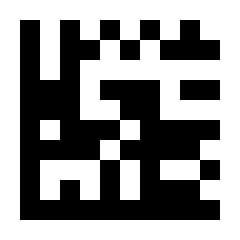
\includegraphics[width=\linewidth]{abbildungen/tag19/mut.png}\\
  \footnotesize\textit{Reines Bitmap}
\end{minipage}\hfill
\begin{minipage}[t]{0.55\linewidth}\centering
  \begin{tikzpicture}[x=7mm, y=-7mm, every node/.style={font=\tiny}]
    \draw[black] (0, 0) rectangle (10, 10);
    \foreach \c in {0,...,9}{ \fill[black] (\c, 9) rectangle (\c+1, 10); }
    \foreach \r in {0,...,8}{ \fill[black] (0, \r) rectangle (1, \r+1); }
    \foreach \c in {0, 2, 4, 6, 8}{ \fill[black] (\c, 0) rectangle (\c+1, 1); }
    \foreach \r in {1, 3, 5, 7}{ \fill[black] (9, \r) rectangle (10, \r+1); }
    \input{abbildungen/tag19/mut_filled_colored}
  \end{tikzpicture}\\
  \footnotesize\textit{UTAH-farbig, schwarze Module = Bit~1}
\end{minipage}
\end{center}

Wenn dein handgemaltes Symbol diesem Bitmap modulweise entspricht
\emph{und} dein Smartphone „MUT" liest: fertig. Falls nicht:
vergleiche modulweise — unterschiedliche Bits markierst du mit
einem dritten Stift, dann radierst und schwärzst du sie passend nach.

% =============================================================
\subsection*{Bonus „GESCHAFFT" — Lösungsweg}
% =============================================================

Größer und länger, aber rechnerisch derselbe Vorgang. 8 Daten-CW im
C40-Modus, 10 ECC-CW, 18 CW gesamt im 14×14-Symbol.

\paragraph{Checkpoint A' — C40-Triplet-Codierung}
\texttt{GESCHAFFT} zerfällt in drei vollständige Triplets:
\texttt{GES}, \texttt{CHA}, \texttt{FFT}. Pro Triplet:
$\mathit{tmp} = V_1 \cdot 1600 + V_2 \cdot 40 + V_3 + 1$, dann
$b_1 = \mathit{tmp} \gg 8$ und $b_2 = \mathit{tmp} \bmod 256$.

\begin{center}
\footnotesize
\setlength{\tabcolsep}{6pt}
\renewcommand{\arraystretch}{1.15}
\begin{tabular}{l|rrr|r|rr}
\toprule
\textbf{Tripel} & $V_1$ & $V_2$ & $V_3$ & $\mathit{tmp}$ & $b_1$ & $b_2$ \\
\midrule
\texttt{GES} & 20 & 18 & 32 & 32753 & 127 & 241 \\
\texttt{CHA} & 16 & 21 & 14 & 26455 & 103 & 87 \\
\texttt{FFT} & 19 & 19 & 33 & 31194 & 121 & 218 \\
\bottomrule
\end{tabular}
\end{center}


C40-Werte: $G{=}14, R{=}28, E{=}18, S{=}32, C{=}16, H{=}21, A{=}14$ \\
\null\hspace{2em}$F{=}19, T{=}33$ \\
(Erinnerung Etappe~18: Buchstabe $X$ hat Wert $14 + (X-A)$.)

\textbf{Daten-CW (mit Latch 230 und Unlatch 254):}
\[ [\,230,\,127,\,241,\,103,\,87,\,121,\,218,\,254\,] \]

\paragraph{Checkpoint B' — Generator-Polynom $g_{10}(x)$}
Zehn Aufbauschritte. Von Grad~1 bis Grad~10 wachsend:

\begin{center}
\footnotesize
\setlength{\tabcolsep}{4pt}
\renewcommand{\arraystretch}{1.15}
\begin{tabular}{r|rrrrrrrrrrr}
\toprule
$g_i(x)$ & $x^{0}$ & $x^{1}$ & $x^{2}$ & $x^{3}$ & $x^{4}$ & $x^{5}$ & $x^{6}$ & $x^{7}$ & $x^{8}$ & $x^{9}$ & $x^{10}$ \\
\midrule
$g_{1}$ & 2 & 1 &  &  &  &  &  &  &  &  &  \\
$g_{2}$ & 8 & 6 & 1 &  &  &  &  &  &  &  &  \\
$g_{3}$ & 64 & 56 & 14 & 1 &  &  &  &  &  &  &  \\
$g_{4}$ & 180 & 183 & 216 & 30 & 1 &  &  &  &  &  &  \\
$g_{5}$ & 228 & 48 & 15 & 111 & 62 & 1 &  &  &  &  &  \\
$g_{6}$ & 219 & 21 & 135 & 119 & 105 & 126 & 1 &  &  &  &  \\
$g_{7}$ & 23 & 68 & 144 & 134 & 240 & 92 & 254 & 1 &  &  &  \\
$g_{8}$ & 73 & 209 & 42 & 154 & 163 & 249 & 210 & 211 & 1 &  &  \\
$g_{9}$ & 52 & 43 & 157 & 200 & 227 & 57 & 117 & 4 & 137 & 1 &  \\
$g_{10}$ & 28 & 24 & 185 & 166 & 223 & 248 & 116 & 255 & 110 & 61 & 1 \\
\bottomrule
\end{tabular}
\end{center}


Endgültige Koeffizienten aufsteigend:
$[28,\,24,\,185,\,166,\,223,\,248,\,116,\,255,\,110,\,61,\,1]$.

\paragraph{Checkpoint C' — RS-Iterationen}
Acht Iterationen mit je 11~Multiplikationen = 88~Stück. Bei jedem
Eintritts-Checkpoint stimmt der Rest-Vektor — wenn deiner abweicht,
kennst du das Iterations-Niveau, ab dem du suchen musst.

\paragraph{Iteration 1 — Faktor $f = 230$}
\textit{Rest vorher:} \texttt{[230, 127, 241, 103, 87, 121, 218, 254, 0, 0, 0, 0, 0, 0, 0, 0, 0, 0]}\par
\begin{center}
\footnotesize
\setlength{\tabcolsep}{4pt}
\renewcommand{\arraystretch}{1.1}
\begin{tabular}{r|rr|rrrr|rrr}
\toprule
$j$ & $g$ & $f$ & $\log g$ & $\log f$ & $\Sigma$ & $\Sigma\bmod 255$ & Pos & vor $\oplus$ Prod & nach \\
\midrule
0 & 1 & 230 & 0 & 68 & 68 & 68 & 0 & 230 $\oplus$ 230 & 0 \\
1 & 61 & 230 & 199 & 68 & 267 & 12 & 1 & 127 $\oplus$ 138 & 245 \\
2 & 110 & 230 & 50 & 68 & 118 & 118 & 2 & 241 $\oplus$ 29 & 236 \\
3 & 255 & 230 & 150 & 68 & 218 & 218 & 3 & 103 $\oplus$ 134 & 225 \\
4 & 116 & 230 & 120 & 68 & 188 & 188 & 4 & 87 $\oplus$ 196 & 147 \\
5 & 248 & 230 & 237 & 68 & 305 & 50 & 5 & 121 $\oplus$ 110 & 23 \\
6 & 223 & 230 & 131 & 68 & 199 & 199 & 6 & 218 $\oplus$ 61 & 231 \\
7 & 166 & 230 & 172 & 68 & 240 & 240 & 7 & 254 $\oplus$ 3 & 253 \\
8 & 185 & 230 & 83 & 68 & 151 & 151 & 8 & 0 $\oplus$ 211 & 211 \\
9 & 24 & 230 & 243 & 68 & 311 & 56 & 9 & 0 $\oplus$ 56 & 56 \\
10 & 28 & 230 & 55 & 68 & 123 & 123 & 10 & 0 $\oplus$ 215 & 215 \\
\bottomrule
\end{tabular}
\end{center}
\textit{Rest nachher:} \texttt{[0, 245, 236, 225, 147, 23, 231, 253, 211, 56, 215, 0, 0, 0, 0, 0, 0, 0]}\par\medskip
\paragraph{Iteration 2 — Faktor $f = 245$}
\textit{Rest vorher:} \texttt{[0, 245, 236, 225, 147, 23, 231, 253, 211, 56, 215, 0, 0, 0, 0, 0, 0, 0]}\par
\begin{center}
\footnotesize
\setlength{\tabcolsep}{4pt}
\renewcommand{\arraystretch}{1.1}
\begin{tabular}{r|rr|rrrr|rrr}
\toprule
$j$ & $g$ & $f$ & $\log g$ & $\log f$ & $\Sigma$ & $\Sigma\bmod 255$ & Pos & vor $\oplus$ Prod & nach \\
\midrule
0 & 1 & 245 & 0 & 156 & 156 & 156 & 1 & 245 $\oplus$ 245 & 0 \\
1 & 61 & 245 & 199 & 156 & 355 & 100 & 2 & 236 $\oplus$ 106 & 134 \\
2 & 110 & 245 & 50 & 156 & 206 & 206 & 3 & 225 $\oplus$ 161 & 64 \\
3 & 255 & 245 & 150 & 156 & 306 & 51 & 4 & 147 $\oplus$ 220 & 79 \\
4 & 116 & 245 & 120 & 156 & 276 & 21 & 5 & 23 $\oplus$ 219 & 204 \\
5 & 248 & 245 & 237 & 156 & 393 & 138 & 6 & 231 $\oplus$ 77 & 170 \\
6 & 223 & 245 & 131 & 156 & 287 & 32 & 7 & 253 $\oplus$ 93 & 160 \\
7 & 166 & 245 & 172 & 156 & 328 & 73 & 8 & 211 $\oplus$ 187 & 104 \\
8 & 185 & 245 & 83 & 156 & 239 & 239 & 9 & 56 $\oplus$ 151 & 175 \\
9 & 24 & 245 & 243 & 156 & 399 & 144 & 10 & 215 $\oplus$ 189 & 106 \\
10 & 28 & 245 & 55 & 156 & 211 & 211 & 11 & 0 $\oplus$ 30 & 30 \\
\bottomrule
\end{tabular}
\end{center}
\textit{Rest nachher:} \texttt{[0, 0, 134, 64, 79, 204, 170, 160, 104, 175, 106, 30, 0, 0, 0, 0, 0, 0]}\par\medskip
\paragraph{Iteration 3 — Faktor $f = 134$}
\textit{Rest vorher:} \texttt{[0, 0, 134, 64, 79, 204, 170, 160, 104, 175, 106, 30, 0, 0, 0, 0, 0, 0]}\par
\begin{center}
\footnotesize
\setlength{\tabcolsep}{4pt}
\renewcommand{\arraystretch}{1.1}
\begin{tabular}{r|rr|rrrr|rrr}
\toprule
$j$ & $g$ & $f$ & $\log g$ & $\log f$ & $\Sigma$ & $\Sigma\bmod 255$ & Pos & vor $\oplus$ Prod & nach \\
\midrule
0 & 1 & 134 & 0 & 218 & 218 & 218 & 2 & 134 $\oplus$ 134 & 0 \\
1 & 61 & 134 & 199 & 218 & 417 & 162 & 3 & 64 $\oplus$ 47 & 111 \\
2 & 110 & 134 & 50 & 218 & 268 & 13 & 4 & 79 $\oplus$ 57 & 118 \\
3 & 255 & 134 & 150 & 218 & 368 & 113 & 5 & 204 $\oplus$ 159 & 83 \\
4 & 116 & 134 & 120 & 218 & 338 & 83 & 6 & 170 $\oplus$ 185 & 19 \\
5 & 248 & 134 & 237 & 218 & 455 & 200 & 7 & 160 $\oplus$ 122 & 218 \\
6 & 223 & 134 & 131 & 218 & 349 & 94 & 8 & 104 $\oplus$ 213 & 189 \\
7 & 166 & 134 & 172 & 218 & 390 & 135 & 9 & 175 $\oplus$ 44 & 131 \\
8 & 185 & 134 & 83 & 218 & 301 & 46 & 10 & 106 $\oplus$ 104 & 2 \\
9 & 24 & 134 & 243 & 218 & 461 & 206 & 11 & 30 $\oplus$ 161 & 191 \\
10 & 28 & 134 & 55 & 218 & 273 & 18 & 12 & 0 $\oplus$ 227 & 227 \\
\bottomrule
\end{tabular}
\end{center}
\textit{Rest nachher:} \texttt{[0, 0, 0, 111, 118, 83, 19, 218, 189, 131, 2, 191, 227, 0, 0, 0, 0, 0]}\par\medskip
\paragraph{Iteration 4 — Faktor $f = 111$}
\textit{Rest vorher:} \texttt{[0, 0, 0, 111, 118, 83, 19, 218, 189, 131, 2, 191, 227, 0, 0, 0, 0, 0]}\par
\begin{center}
\footnotesize
\setlength{\tabcolsep}{4pt}
\renewcommand{\arraystretch}{1.1}
\begin{tabular}{r|rr|rrrr|rrr}
\toprule
$j$ & $g$ & $f$ & $\log g$ & $\log f$ & $\Sigma$ & $\Sigma\bmod 255$ & Pos & vor $\oplus$ Prod & nach \\
\midrule
0 & 1 & 111 & 0 & 207 & 207 & 207 & 3 & 111 $\oplus$ 111 & 0 \\
1 & 61 & 111 & 199 & 207 & 406 & 151 & 4 & 118 $\oplus$ 211 & 165 \\
2 & 110 & 111 & 50 & 207 & 257 & 2 & 5 & 83 $\oplus$ 4 & 87 \\
3 & 255 & 111 & 150 & 207 & 357 & 102 & 6 & 19 $\oplus$ 133 & 150 \\
4 & 116 & 111 & 120 & 207 & 327 & 72 & 7 & 218 $\oplus$ 203 & 17 \\
5 & 248 & 111 & 237 & 207 & 444 & 189 & 8 & 189 $\oplus$ 165 & 24 \\
6 & 223 & 111 & 131 & 207 & 338 & 83 & 9 & 131 $\oplus$ 185 & 58 \\
7 & 166 & 111 & 172 & 207 & 379 & 124 & 10 & 2 $\oplus$ 131 & 129 \\
8 & 185 & 111 & 83 & 207 & 290 & 35 & 11 & 191 $\oplus$ 178 & 13 \\
9 & 24 & 111 & 243 & 207 & 450 & 195 & 12 & 227 $\oplus$ 17 & 242 \\
10 & 28 & 111 & 55 & 207 & 262 & 7 & 13 & 0 $\oplus$ 128 & 128 \\
\bottomrule
\end{tabular}
\end{center}
\textit{Rest nachher:} \texttt{[0, 0, 0, 0, 165, 87, 150, 17, 24, 58, 129, 13, 242, 128, 0, 0, 0, 0]}\par\medskip
\paragraph{Iteration 5 — Faktor $f = 165$}
\textit{Rest vorher:} \texttt{[0, 0, 0, 0, 165, 87, 150, 17, 24, 58, 129, 13, 242, 128, 0, 0, 0, 0]}\par
\begin{center}
\footnotesize
\setlength{\tabcolsep}{4pt}
\renewcommand{\arraystretch}{1.1}
\begin{tabular}{r|rr|rrrr|rrr}
\toprule
$j$ & $g$ & $f$ & $\log g$ & $\log f$ & $\Sigma$ & $\Sigma\bmod 255$ & Pos & vor $\oplus$ Prod & nach \\
\midrule
0 & 1 & 165 & 0 & 189 & 189 & 189 & 4 & 165 $\oplus$ 165 & 0 \\
1 & 61 & 165 & 199 & 189 & 388 & 133 & 5 & 87 $\oplus$ 11 & 92 \\
2 & 110 & 165 & 50 & 189 & 239 & 239 & 6 & 150 $\oplus$ 151 & 1 \\
3 & 255 & 165 & 150 & 189 & 339 & 84 & 7 & 17 $\oplus$ 95 & 78 \\
4 & 116 & 165 & 120 & 189 & 309 & 54 & 8 & 24 $\oplus$ 14 & 22 \\
5 & 248 & 165 & 237 & 189 & 426 & 171 & 9 & 58 $\oplus$ 83 & 105 \\
6 & 223 & 165 & 131 & 189 & 320 & 65 & 10 & 129 $\oplus$ 193 & 64 \\
7 & 166 & 165 & 172 & 189 & 361 & 106 & 11 & 13 $\oplus$ 21 & 24 \\
8 & 185 & 165 & 83 & 189 & 272 & 17 & 12 & 242 $\oplus$ 231 & 21 \\
9 & 24 & 165 & 243 & 189 & 432 & 177 & 13 & 128 $\oplus$ 254 & 126 \\
10 & 28 & 165 & 55 & 189 & 244 & 244 & 14 & 0 $\oplus$ 48 & 48 \\
\bottomrule
\end{tabular}
\end{center}
\textit{Rest nachher:} \texttt{[0, 0, 0, 0, 0, 92, 1, 78, 22, 105, 64, 24, 21, 126, 48, 0, 0, 0]}\par\medskip
\paragraph{Iteration 6 — Faktor $f = 92$}
\textit{Rest vorher:} \texttt{[0, 0, 0, 0, 0, 92, 1, 78, 22, 105, 64, 24, 21, 126, 48, 0, 0, 0]}\par
\begin{center}
\footnotesize
\setlength{\tabcolsep}{4pt}
\renewcommand{\arraystretch}{1.1}
\begin{tabular}{r|rr|rrrr|rrr}
\toprule
$j$ & $g$ & $f$ & $\log g$ & $\log f$ & $\Sigma$ & $\Sigma\bmod 255$ & Pos & vor $\oplus$ Prod & nach \\
\midrule
0 & 1 & 92 & 0 & 30 & 30 & 30 & 5 & 92 $\oplus$ 92 & 0 \\
1 & 61 & 92 & 199 & 30 & 229 & 229 & 6 & 1 $\oplus$ 80 & 81 \\
2 & 110 & 92 & 50 & 30 & 80 & 80 & 7 & 78 $\oplus$ 164 & 234 \\
3 & 255 & 92 & 150 & 30 & 180 & 180 & 8 & 22 $\oplus$ 51 & 37 \\
4 & 116 & 92 & 120 & 30 & 150 & 150 & 9 & 105 $\oplus$ 255 & 150 \\
5 & 248 & 92 & 237 & 30 & 267 & 12 & 10 & 64 $\oplus$ 138 & 202 \\
6 & 223 & 92 & 131 & 30 & 161 & 161 & 11 & 24 $\oplus$ 129 & 153 \\
7 & 166 & 92 & 172 & 30 & 202 & 202 & 12 & 21 $\oplus$ 197 & 208 \\
8 & 185 & 92 & 83 & 30 & 113 & 113 & 13 & 126 $\oplus$ 159 & 225 \\
9 & 24 & 92 & 243 & 30 & 273 & 18 & 14 & 48 $\oplus$ 227 & 211 \\
10 & 28 & 92 & 55 & 30 & 85 & 85 & 15 & 0 $\oplus$ 190 & 190 \\
\bottomrule
\end{tabular}
\end{center}
\textit{Rest nachher:} \texttt{[0, 0, 0, 0, 0, 0, 81, 234, 37, 150, 202, 153, 208, 225, 211, 190, 0, 0]}\par\medskip
\paragraph{Iteration 7 — Faktor $f = 81$}
\textit{Rest vorher:} \texttt{[0, 0, 0, 0, 0, 0, 81, 234, 37, 150, 202, 153, 208, 225, 211, 190, 0, 0]}\par
\begin{center}
\footnotesize
\setlength{\tabcolsep}{4pt}
\renewcommand{\arraystretch}{1.1}
\begin{tabular}{r|rr|rrrr|rrr}
\toprule
$j$ & $g$ & $f$ & $\log g$ & $\log f$ & $\Sigma$ & $\Sigma\bmod 255$ & Pos & vor $\oplus$ Prod & nach \\
\midrule
0 & 1 & 81 & 0 & 86 & 86 & 86 & 6 & 81 $\oplus$ 81 & 0 \\
1 & 61 & 81 & 199 & 86 & 285 & 30 & 7 & 234 $\oplus$ 92 & 182 \\
2 & 110 & 81 & 50 & 86 & 136 & 136 & 8 & 37 $\oplus$ 88 & 125 \\
3 & 255 & 81 & 150 & 86 & 236 & 236 & 9 & 150 $\oplus$ 124 & 234 \\
4 & 116 & 81 & 120 & 86 & 206 & 206 & 10 & 202 $\oplus$ 161 & 107 \\
5 & 248 & 81 & 237 & 86 & 323 & 68 & 11 & 153 $\oplus$ 230 & 127 \\
6 & 223 & 81 & 131 & 86 & 217 & 217 & 12 & 208 $\oplus$ 67 & 147 \\
7 & 166 & 81 & 172 & 86 & 258 & 3 & 13 & 225 $\oplus$ 8 & 233 \\
8 & 185 & 81 & 83 & 86 & 169 & 169 & 14 & 211 $\oplus$ 201 & 26 \\
9 & 24 & 81 & 243 & 86 & 329 & 74 & 15 & 190 $\oplus$ 91 & 229 \\
10 & 28 & 81 & 55 & 86 & 141 & 141 & 16 & 0 $\oplus$ 50 & 50 \\
\bottomrule
\end{tabular}
\end{center}
\textit{Rest nachher:} \texttt{[0, 0, 0, 0, 0, 0, 0, 182, 125, 234, 107, 127, 147, 233, 26, 229, 50, 0]}\par\medskip
\paragraph{Iteration 8 — Faktor $f = 182$}
\textit{Rest vorher:} \texttt{[0, 0, 0, 0, 0, 0, 0, 182, 125, 234, 107, 127, 147, 233, 26, 229, 50, 0]}\par
\begin{center}
\footnotesize
\setlength{\tabcolsep}{4pt}
\renewcommand{\arraystretch}{1.1}
\begin{tabular}{r|rr|rrrr|rrr}
\toprule
$j$ & $g$ & $f$ & $\log g$ & $\log f$ & $\Sigma$ & $\Sigma\bmod 255$ & Pos & vor $\oplus$ Prod & nach \\
\midrule
0 & 1 & 182 & 0 & 75 & 75 & 75 & 7 & 182 $\oplus$ 182 & 0 \\
1 & 61 & 182 & 199 & 75 & 274 & 19 & 8 & 125 $\oplus$ 235 & 150 \\
2 & 110 & 182 & 50 & 75 & 125 & 125 & 9 & 234 $\oplus$ 43 & 193 \\
3 & 255 & 182 & 150 & 75 & 225 & 225 & 10 & 107 $\oplus$ 5 & 110 \\
4 & 116 & 182 & 120 & 75 & 195 & 195 & 11 & 127 $\oplus$ 17 & 110 \\
5 & 248 & 182 & 237 & 75 & 312 & 57 & 12 & 147 $\oplus$ 112 & 227 \\
6 & 223 & 182 & 131 & 75 & 206 & 206 & 13 & 233 $\oplus$ 161 & 72 \\
7 & 166 & 182 & 172 & 75 & 247 & 247 & 14 & 26 $\oplus$ 173 & 183 \\
8 & 185 & 182 & 83 & 75 & 158 & 158 & 15 & 229 $\oplus$ 163 & 70 \\
9 & 24 & 182 & 243 & 75 & 318 & 63 & 16 & 50 $\oplus$ 123 & 73 \\
10 & 28 & 182 & 55 & 75 & 130 & 130 & 17 & 0 $\oplus$ 249 & 249 \\
\bottomrule
\end{tabular}
\end{center}
\textit{Rest nachher:} \texttt{[0, 0, 0, 0, 0, 0, 0, 0, 150, 193, 110, 110, 227, 72, 183, 70, 73, 249]}\par\medskip


\paragraph{Checkpoint D' — Finale Codewords}
\textbf{ECC: $[150, 193, 110, 110, 227, 72, 183, 70, 73, 249]$}.
Vollständige 18er-Folge:
\[
  [\,230,\,127,\,241,\,103,\,87,\,121,\,218,\,254,\,|
\]
\[
  150,\,193,\,110,\,110,\,227,\,72,\,183,\,70,\,73,\,249\,]
\]

\paragraph{Checkpoint E' — Bit-Zerlegung}

\begin{center}
\footnotesize
\setlength{\tabcolsep}{4pt}
\renewcommand{\arraystretch}{1.2}
\begin{tabular}{r|r|cccccccc}
\toprule
\textbf{CW} & \textbf{Wert} & \textbf{1} & \textbf{2} & \textbf{3} & \textbf{4} & \textbf{5} & \textbf{6} & \textbf{7} & \textbf{8} \\
& & \tiny 128 & \tiny 64 & \tiny 32 & \tiny 16 & \tiny 8 & \tiny 4 & \tiny 2 & \tiny 1 \\
\midrule
1 & 230 & 1 & 1 & 1 & 0 & 0 & 1 & 1 & 0 \\
2 & 127 & 0 & 1 & 1 & 1 & 1 & 1 & 1 & 1 \\
3 & 241 & 1 & 1 & 1 & 1 & 0 & 0 & 0 & 1 \\
4 & 103 & 0 & 1 & 1 & 0 & 0 & 1 & 1 & 1 \\
5 & 87 & 0 & 1 & 0 & 1 & 0 & 1 & 1 & 1 \\
6 & 121 & 0 & 1 & 1 & 1 & 1 & 0 & 0 & 1 \\
7 & 218 & 1 & 1 & 0 & 1 & 1 & 0 & 1 & 0 \\
8 & 254 & 1 & 1 & 1 & 1 & 1 & 1 & 1 & 0 \\
9 & 150 & 1 & 0 & 0 & 1 & 0 & 1 & 1 & 0 \\
10 & 193 & 1 & 1 & 0 & 0 & 0 & 0 & 0 & 1 \\
11 & 110 & 0 & 1 & 1 & 0 & 1 & 1 & 1 & 0 \\
12 & 110 & 0 & 1 & 1 & 0 & 1 & 1 & 1 & 0 \\
13 & 227 & 1 & 1 & 1 & 0 & 0 & 0 & 1 & 1 \\
14 & 72 & 0 & 1 & 0 & 0 & 1 & 0 & 0 & 0 \\
15 & 183 & 1 & 0 & 1 & 1 & 0 & 1 & 1 & 1 \\
16 & 70 & 0 & 1 & 0 & 0 & 0 & 1 & 1 & 0 \\
17 & 73 & 0 & 1 & 0 & 0 & 1 & 0 & 0 & 1 \\
18 & 249 & 1 & 1 & 1 & 1 & 1 & 0 & 0 & 1 \\
\bottomrule
\end{tabular}
\end{center}


\paragraph{Checkpoint F' — Platzierung im 12×12-Datenbereich}

\begin{center}
\footnotesize
\setlength{\tabcolsep}{2pt}
\renewcommand{\arraystretch}{1.05}
\begin{tabular}{c|cccccccccccc}
\toprule
$r\backslash c$ & 1 & 2 & 3 & 4 & 5 & 6 & 7 & 8 & 9 & 10 & 11 & 12 \\
\midrule
1 & 2/1 & 2/2 & 3/6 & 3/7 & 3/8 & 4/3 & 4/4 & 4/5 & 13/1 & 13/2 & 8/4 & 8/5 \\
2 & 2/3 & 2/4 & 2/5 & 5/1 & 5/2 & 4/6 & 4/7 & 4/8 & 13/3 & 13/4 & 13/5 & 8/6 \\
3 & 2/6 & 2/7 & 2/8 & 5/3 & 5/4 & 5/5 & 12/1 & 12/2 & 13/6 & 13/7 & 13/8 & 8/7 \\
4 & 1/5 & 6/1 & 6/2 & 5/6 & 5/7 & 5/8 & 12/3 & 12/4 & 12/5 & 14/1 & 14/2 & 8/8 \\
5 & 1/8 & 6/3 & 6/4 & 6/5 & 11/1 & 11/2 & 12/6 & 12/7 & 12/8 & 14/3 & 14/4 & 14/5 \\
6 & 7/2 & 6/6 & 6/7 & 6/8 & 11/3 & 11/4 & 11/5 & 15/1 & 15/2 & 14/6 & 14/7 & 14/8 \\
7 & 7/4 & 7/5 & 10/1 & 10/2 & 11/6 & 11/7 & 11/8 & 15/3 & 15/4 & 15/5 & 1/1 & 1/2 \\
8 & 7/7 & 7/8 & 10/3 & 10/4 & 10/5 & 16/1 & 16/2 & 15/6 & 15/7 & 15/8 & 1/3 & 1/4 \\
9 & 9/1 & 9/2 & 10/6 & 10/7 & 10/8 & 16/3 & 16/4 & 16/5 & 18/1 & 18/2 & 1/6 & 1/7 \\
10 & 9/3 & 9/4 & 9/5 & 17/1 & 17/2 & 16/6 & 16/7 & 16/8 & 18/3 & 18/4 & 18/5 & 7/1 \\
11 & 9/6 & 9/7 & 9/8 & 17/3 & 17/4 & 17/5 & 3/1 & 3/2 & 18/6 & 18/7 & 18/8 & 7/3 \\
12 & 8/1 & 8/2 & 8/3 & 17/6 & 17/7 & 17/8 & 3/3 & 3/4 & 3/5 & 4/1 & 4/2 & 7/6 \\
\bottomrule
\end{tabular}
\end{center}


\paragraph{Checkpoint G' — Finales Bitmap}

\begin{center}
\begin{minipage}[t]{0.32\linewidth}\centering
  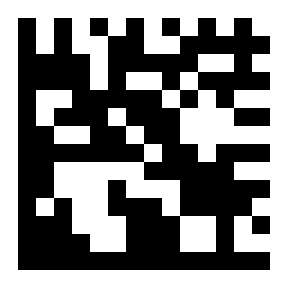
\includegraphics[width=\linewidth]{abbildungen/tag19/geschafft.png}\\
  \footnotesize\textit{Reines Bitmap}
\end{minipage}\hfill
\begin{minipage}[t]{0.62\linewidth}\centering
  \begin{tikzpicture}[x=5.5mm, y=-5.5mm, every node/.style={font=\tiny}]
    \draw[black] (0, 0) rectangle (14, 14);
    \foreach \c in {0,...,13}{ \fill[black] (\c, 13) rectangle (\c+1, 14); }
    \foreach \r in {0,...,12}{ \fill[black] (0, \r) rectangle (1, \r+1); }
    \foreach \c in {0, 2, 4, 6, 8, 10, 12}{
      \fill[black] (\c, 0) rectangle (\c+1, 1);
    }
    \foreach \r in {1, 3, 5, 7, 9, 11}{
      \fill[black] (13, \r) rectangle (14, \r+1);
    }
    \input{abbildungen/tag19/geschafft_filled_colored}
  \end{tikzpicture}\\
  \footnotesize\textit{UTAH-farbig, schwarze Module = Bit~1}
\end{minipage}
\end{center}

Wenn dein handgemaltes 14×14-Symbol diesem Bitmap entspricht und das
Smartphone „GESCHAFFT" liest, hast du im Praktikum eine Datamatrix
\emph{komplett von Hand} erzeugt. Reed-Solomon, GF(256), Annex~F,
C40 — alles eigene Bleistift-Arbeit. Glückwunsch.
